

\chapter{Iteration}

This chapter is about iteration, which is the ability to run
a block of statements repeatedly.  We saw a kind of iteration,
using recursion, in Section~\ref{recursion}.
We saw another kind, using a {\tt for} loop,
in Section~\ref{repetition}.  In this chapter we'll see yet another
kind, using a {\tt while} statement.
But first I want to say a little more about variable assignment.


\section{Reassignment}
\index{assignment}
\index{statement!assignment}
\index{reassignment}

As you may have discovered, it is legal to make more than one
assignment to the same variable.  A new assignment makes an existing
variable refer to a new value (and stop referring to the old value).

\begin{verbatim}
>>> x = 5
>>> x
5
>>> x = 7
>>> x
7
\end{verbatim}
%
The first time we display
{\tt x}, its value is 5; the second time, its
value is 7.

Figure~\ref{fig.assign2} shows what {\bf reassignment} looks
like in a state diagram. \index{state diagram} \index{diagram!state}

At this point I want to address a common source of
confusion.
Because Python uses the equal sign ({\tt =}) for assignment, it is
tempting to interpret a statement like {\tt a = b} as a
mathematical
proposition of equality; that is, the claim that {\tt a} and
{\tt b} are equal.  But this interpretation is wrong.
\index{equality and assignment}

First, equality is a symmetric relationship and assignment is not.  For
example, in mathematics, if $a=7$ then $7=a$.  But in Python, the
statement {\tt a = 7} is legal and {\tt 7 = a} is not.

Also, in mathematics, a proposition of equality is either true or
false for all time.  If $a=b$ now, then $a$ will always equal $b$.
In Python, an assignment statement can make two variables equal, but
they don't have to stay that way:

\begin{verbatim}
>>> a = 5
>>> b = a    # a and b are now equal
>>> a = 3    # a and b are no longer equal
>>> b
5
\end{verbatim}
%
The third line changes the value of {\tt a} but does not change the
value of {\tt b}, so they are no longer equal.

Reassigning variables is often useful, but you should use it
with caution.  If the values of variables change frequently, it can
make the code difficult to read and debug.

\begin{figure}
\centerline
{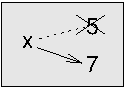
\includegraphics[scale=0.8]{../source/figs/assign2.pdf}}
\caption{State diagram.}
\label{fig.assign2}
\end{figure}



\section{Updating variables}
\label{update}

\index{update}
\index{variable!updating}

A common kind of reassignment is an {\bf update},
where the new value of the variable depends on the old.

\begin{verbatim}
>>> x = x + 1
\end{verbatim}
%
This means ``get the current value of {\tt x}, add one, and then
update {\tt x} with the new value.''

If you try to update a variable that doesn't exist, you get an
error, because Python evaluates the right side before it assigns
a value to {\tt x}:

\begin{verbatim}
>>> x = x + 1
NameError: name 'x' is not defined
\end{verbatim}
%
Before you can update a variable, you have to {\bf initialize}
it, usually with a simple assignment:
\index{initialization (before update)}

\begin{verbatim}
>>> x = 0
>>> x = x + 1
\end{verbatim}
%
Updating a variable by adding 1 is called an {\bf increment};
subtracting 1 is called a {\bf decrement}.
\index{increment}
\index{decrement}




\section{The {\tt while} statement}
\index{statement!while}
\index{while loop}
\index{loop!while}
\index{iteration}

Computers are often used to automate repetitive tasks.  Repeating
identical or similar tasks without making errors is something that
computers do well and people do poorly.  In a computer program,
repetition is also called {\bf iteration}.

We have already seen two functions, {\tt countdown} and
\verb"print_n", that iterate using recursion.  Because iteration is so
common, Python provides language features to make it easier.
One is the {\tt for} statement we saw in Section~\ref{repetition}.
We'll get back to that later.

Another is the {\tt while} statement.  Here is a version of {\tt
countdown} that uses a {\tt while} statement:

\begin{verbatim}
def countdown(n):
    while n > 0:
        print(n)
        n = n - 1
    print('Blastoff!')
\end{verbatim}
%
You can almost read the {\tt while} statement as if it were English.
It means, ``While {\tt n} is greater than 0,
display the value of {\tt n} and then decrement
{\tt n}.  When you get to 0, display the word {\tt Blastoff!}''
\index{flow of execution}

More formally, here is the flow of execution for a {\tt while} statement:

\begin{enumerate}

\item Determine whether the condition is true or false.

\item If false, exit the {\tt while} statement
and continue execution at the next statement.

\item If the condition is true, run the
body and then go back to step 1.

\end{enumerate}

This type of flow is called a loop because the third step
loops back around to the top.
\index{condition}
\index{loop}
\index{body}

The body of the loop should change the value of one or more variables
so that the condition becomes false eventually and the loop
terminates.  Otherwise the loop will repeat forever, which is called
an {\bf infinite loop}.  An endless source of amusement for computer
scientists is the observation that the directions on shampoo,
``Lather, rinse, repeat'', are an infinite loop.
\index{infinite loop}
\index{loop!infinite}

In the case of {\tt countdown}, we can prove that the loop
terminates: if {\tt n} is zero or negative, the loop never runs.
Otherwise, {\tt n} gets smaller each time through the
loop, so eventually we have to get to 0.

For some other loops, it is not so easy to tell.  For example:

\begin{verbatim}
def sequence(n):
    while n != 1:
        print(n)
        if n % 2 == 0:        # n is even
            n = n / 2
        else:                 # n is odd
            n = n*3 + 1
\end{verbatim}
%
The condition for this loop is {\tt n != 1}, so the loop will continue
until {\tt n} is {\tt 1}, which makes the condition false.

Each time through the loop, the program outputs the value of {\tt n}
and then checks whether it is even or odd.  If it is even, {\tt n} is
divided by 2.  If it is odd, the value of {\tt n} is replaced with
{\tt n*3 + 1}. For example, if the argument passed to {\tt sequence}
is 3, the resulting values of {\tt n} are 3, 10, 5, 16, 8, 4, 2, 1.

Since {\tt n} sometimes increases and sometimes decreases, there is no
obvious proof that {\tt n} will ever reach 1, or that the program
terminates.  For some particular values of {\tt n}, we can prove
termination.  For example, if the starting value is a power of two,
{\tt n} will be even every time through the loop
until it reaches 1. The previous example ends with such a sequence,
starting with 16.
\index{Collatz conjecture}

The hard question is whether we can prove that this program terminates
for {\em all} positive values of {\tt n}.  So far, no one has
been able to prove it {\em or} disprove it!  (See
  \url{http://en.wikipedia.org/wiki/Collatz_conjecture}.)

As an exercise, rewrite the function \verb"print_n" from
Section~\ref{recursion} using iteration instead of recursion.


\section{{\tt break}}
\index{break statement}
\index{statement!break}

Sometimes you don't know it's time to end a loop until you get half
way through the body.  In that case you can use the {\tt break}
statement to jump out of the loop.

For example, suppose you want to take input from the user until they
type {\tt done}.  You could write:

\begin{verbatim}
while True:
    line = input('> ')
    if line == 'done':
        break
    print(line)

print('Done!')
\end{verbatim}
%
The loop condition is {\tt True}, which is always true, so the
loop runs until it hits the break statement.

Each time through, it prompts the user with an angle bracket.
If the user types {\tt done}, the {\tt break} statement exits
the loop.  Otherwise the program echoes whatever the user types
and goes back to the top of the loop.  Here's a sample run:

\begin{verbatim}
> not done
not done
> done
Done!
\end{verbatim}
%
This way of writing {\tt while} loops is common because you
can check the condition anywhere in the loop (not just at the
top) and you can express the stop condition affirmatively
(``stop when this happens'') rather than negatively (``keep going
until that happens'').


\section{Square roots}
\label{squareroot}
\index{square root}

Loops are often used in programs that compute
numerical results by starting with an approximate answer and
iteratively improving it.
\index{Newton's method}

For example, one way of computing square roots is Newton's method.
Suppose that you want to know the square root of $a$.  If you start
with almost any estimate, $x$, you can compute a better
estimate with the following formula:

\[ y = \frac{x + a/x}{2} \]
%
For example, if $a$ is 4 and $x$ is 3:

\begin{verbatim}
>>> a = 4
>>> x = 3
>>> y = (x + a/x) / 2
>>> y
2.16666666667
\end{verbatim}
%
The result is closer to the correct answer ($\sqrt{4} = 2$).  If we
repeat the process with the new estimate, it gets even closer:

\begin{verbatim}
>>> x = y
>>> y = (x + a/x) / 2
>>> y
2.00641025641
\end{verbatim}
%
After a few more updates, the estimate is almost exact:
\index{update}

\begin{verbatim}
>>> x = y
>>> y = (x + a/x) / 2
>>> y
2.00001024003
>>> x = y
>>> y = (x + a/x) / 2
>>> y
2.00000000003
\end{verbatim}
%
In general we don't know ahead of time how many steps it takes
to get to the right answer, but we know when we get there
because the estimate
stops changing:

\begin{verbatim}
>>> x = y
>>> y = (x + a/x) / 2
>>> y
2.0
>>> x = y
>>> y = (x + a/x) / 2
>>> y
2.0
\end{verbatim}
%
When {\tt y == x}, we can stop.  Here is a loop that starts
with an initial estimate, {\tt x}, and improves it until it
stops changing:

\begin{verbatim}
while True:
    print(x)
    y = (x + a/x) / 2
    if y == x:
        break
    x = y
\end{verbatim}
%
For most values of {\tt a} this works fine, but in general it is
dangerous to test {\tt float} equality.
Floating-point values are only approximately right:
most rational numbers, like $1/3$, and irrational numbers, like
$\sqrt{2}$, can't be represented exactly with a {\tt float}.
\index{floating-point}
\index{epsilon}

Rather than checking whether {\tt x} and {\tt y} are exactly equal, it
is safer to use the built-in function {\tt abs} to compute the
absolute value, or magnitude, of the difference between them:

\begin{verbatim}
    if abs(y-x) < epsilon:
        break
\end{verbatim}
%
Where \verb"epsilon" has a value like {\tt 0.0000001} that
determines how close is close enough.


\section{Algorithms}
\index{algorithm}

Newton's method is an example of an {\bf algorithm}: it is a
mechanical process for solving a category of problems (in this
case, computing square roots).

To understand what an algorithm is, it might help to start with
something that is not an algorithm.  When you learned to multiply
single-digit numbers, you probably memorized the multiplication table.
In effect, you memorized 100 specific solutions.  That kind of
knowledge is not algorithmic.

But if you were ``lazy'', you might have learned a few
tricks.  For example, to find the product of $n$ and 9, you can
write $n-1$ as the first digit and $10-n$ as the second
digit.  This trick is a general solution for multiplying any
single-digit number by 9.  That's an algorithm!
\index{addition with carrying}
\index{carrying, addition with}
\index{subtraction!with borrowing}
\index{borrowing, subtraction with}

Similarly, the techniques you learned for addition with carrying,
subtraction with borrowing, and long division are all algorithms.  One
of the characteristics of algorithms is that they do not require any
intelligence to carry out.  They are mechanical processes where
each step follows from the last according to a simple set of rules.

Executing algorithms is boring, but designing them is interesting,
intellectually challenging, and a central part of computer science.

Some of the things that people do naturally, without difficulty or
conscious thought, are the hardest to express algorithmically.
Understanding natural language is a good example.  We all do it, but
so far no one has been able to explain {\em how} we do it, at least
not in the form of an algorithm.


\section{Debugging}
\label{bisectbug}

As you start writing bigger programs, you might find yourself
spending more time debugging.  More code means more chances to
make an error and more places for bugs to hide.
\index{debugging!by bisection}
\index{bisection, debugging by}

One way to cut your debugging time is ``debugging by bisection''.
For example, if there are 100 lines in your program and you
check them one at a time, it would take 100 steps.

Instead, try to break the problem in half.  Look at the middle
of the program, or near it, for an intermediate value you
can check.  Add a {\tt print} statement (or something else
that has a verifiable effect) and run the program.

If the mid-point check is incorrect, there must be a problem in the
first half of the program.  If it is correct, the problem is
in the second half.

Every time you perform a check like this, you halve the number of
lines you have to search.  After six steps (which is fewer than 100),
you would be down to one or two lines of code, at least in theory.

In practice it is not always clear what
the ``middle of the program'' is and not always possible to
check it.  It doesn't make sense to count lines and find the
exact midpoint.  Instead, think about places
in the program where there might be errors and places where it
is easy to put a check.  Then choose a spot where you
think the chances are about the same that the bug is before
or after the check.




\section{Glossary}

\begin{description}

\item[reassignment:] Assigning a new value to a variable that
already exists.
\index{reassignment}

\item[update:] An assignment where the new value of the variable
depends on the old.
\index{update}

\item[initialization:] An assignment that gives an initial value to
a variable that will be updated.
\index{initialization!variable}

\item[increment:] An update that increases the value of a variable
(often by one).
\index{increment}

\item[decrement:] An update that decreases the value of a variable.
\index{decrement}

\item[iteration:] Repeated execution of a set of statements using
either a recursive function call or a loop.
\index{iteration}

\item[infinite loop:] A loop in which the terminating condition is
never satisfied.
\index{infinite loop}

\item[algorithm:]  A general process for solving a category of
problems.
\index{algorithm}

\end{description}


\section{Exercises}

\begin{exercise}
\index{algorithm!square root}

Copy the loop from Section~\ref{squareroot}
and encapsulate it in a function called
\verb"mysqrt" that takes {\tt a} as a parameter, chooses a
reasonable value of {\tt x}, and returns an estimate of the square
root of {\tt a}.  \index{encapsulation}

To test it, write a function named \verb"test_square_root"
that prints a table like this:

\begin{verbatim}
a   mysqrt(a)     math.sqrt(a)  diff
-   ---------     ------------  ----
1.0 1.0           1.0           0.0
2.0 1.41421356237 1.41421356237 2.22044604925e-16
3.0 1.73205080757 1.73205080757 0.0
4.0 2.0           2.0           0.0
5.0 2.2360679775  2.2360679775  0.0
6.0 2.44948974278 2.44948974278 0.0
7.0 2.64575131106 2.64575131106 0.0
8.0 2.82842712475 2.82842712475 4.4408920985e-16
9.0 3.0           3.0           0.0
\end{verbatim}
%
The first column is a number, $a$; the second column is the square
root of $a$ computed with \verb"mysqrt"; the third column is the
square root computed by {\tt math.sqrt}; the fourth column is the
absolute value of the difference between the two estimates.
\end{exercise}


\begin{exercise}
\index{eval function}
\index{function!eval}

The built-in function {\tt eval} takes a string and evaluates
it using the Python interpreter.  For example:

\begin{verbatim}
>>> eval('1 + 2 * 3')
7
>>> import math
>>> eval('math.sqrt(5)')
2.2360679774997898
>>> eval('type(math.pi)')
<class 'float'>
\end{verbatim}
%
Write a function called \verb"eval_loop" that iteratively
prompts the user, takes the resulting input and evaluates
it using {\tt eval}, and prints the result.

It should continue until the user enters \verb"'done'", and then
return the value of the last expression it evaluated.

\end{exercise}


\begin{exercise}
\index{Ramanujan, Srinivasa}

The mathematician Srinivasa Ramanujan found an
infinite series
that can be used to generate a numerical
approximation of $1 / \pi$:
\index{pi}

\[ \frac{1}{\pi} = \frac{2\sqrt{2}}{9801}
\sum^\infty_{k=0} \frac{(4k)!(1103+26390k)}{(k!)^4 396^{4k}} \]

Write a function called \verb"estimate_pi" that uses this formula
to compute and return an estimate of $\pi$.  It should use a {\tt while}
loop to compute terms of the summation until the last term is
smaller than {\tt 1e-15} (which is Python notation for $10^{-15}$).
You can check the result by comparing it to {\tt math.pi}.

Solution: \url{http://thinkpython2.com/code/pi.py}.

\end{exercise}
